  \begin{figure}
	\centering
	% \includegraphics[width=\linewidth]{fig/design/prepare.drawio.pdf}
	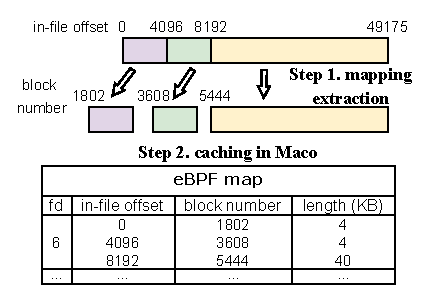
\includegraphics[width=0.9\linewidth]{fig/design/extractMap.pdf}
	%	\vspace{-1ex}
	\caption{An Illustration of \odes's Maco.}% Reorganizing Per-file Mappings}
\label{fig:prepare}
\vspace{-3ex}
\end{figure}

\subsection{Donor-Based Online Space Allocation}
\label{sec:design:donor}

Dynamically growing log files are also common in databases.
Unlike preallocated files, their offset-to-block mappings may change as the
file expands, making it difficult for \odes to cache the mappings while
avoiding costly allocation and journaling on the write critical path.
To address this issue, \odes develops a preallocation-like strategy based on
a \emph{donor pool} and Ext4's \emph{move-extent}
feature~\cite{ext4moveextent}.

\textbf{Donor pool.}
\odes preallocates a pool of donor files containing a large contiguous space of blocks with prefilling zeros and registers their mappings in the Maco structure in advance. These pre-reserved ranges allow \odes to supply space to growing log files without invoking Ext4's normal block allocation on each append.

\textbf{Moving extents.}
Ext4 originally uses \emph{move-extent} for online
defragmentation~\cite{ext4moveextent}. It exchanges extent mappings between
two files without moving the mappings through the normal allocation path if both files do not have   valid data stored in exchanged extents.
\odes repurposes this interface for online space allocation.
For a growing log file, \odes reserves an unused tail range.
When the file requires additional space, \odes exchanges this tail range
with a contiguous range from a donor file and updates the Maco mappings
accordingly. The newly received range then becomes part of the log file, with its end serving as the new tail.


\begin{figure}
    \centering
    \scalebox{0.75}{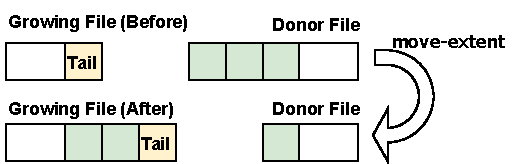
\includegraphics[width=\linewidth]{fig/design/move_extent.pdf}}
    \caption{An illustration of how \odes uses \emph{move-extent} to expand
    a growing log file.}
    \label{fig:des:move_extent}
    \vspace{-3ex}
\end{figure}

\autoref{fig:des:move_extent} illustrates this process.
To amortize the cost of each transfer, \odes moves a contiguous range larger
than a typical logging write. A lightweight monitor maintains the moving
average of logging I/O sizes, and \odes empirically sets the transfer size to
four times this average. The donor pool is replenished in the background
when its free space falls below a threshold, and unused transferred blocks
are returned to their donor file when the log file is closed.

If the donor pool cannot satisfy an allocation request or a \emph{move-extent} operation fails, \odes falls back to Ext4's normal allocation path. Moreover, because \odes prepares extents asynchronously
through io\_uring, a write may arrive before the corresponding
\emph{move-extent} completes. In this case, the write waits for completion
before using the new mapping, preventing it from observing a partially
updated mapping.


\subsection{Optimizations and Discussions}
\label{sec:design:discussion}

\textbf{Optimizations.}
\odes employs two optimizations.
First, it uses io\_uring~\cite{iouring,ioctlWik84:online} to asynchronously
prepare extents for growing log files while current logging writes proceed,
thereby moving most \emph{move-extent} overhead off the critical path.
Second, \odes partitions the Maco structure and donor pool into per-core
structures to reduce contention and improve scalability.

\textbf{Crash consistency.}
\odes changes only the I/O path while preserving the ordering and persistence
semantics expected by the database. It writes to device blocks obtained from
Ext4's extent tree and waits for write and \texttt{fdatasync} completion
before returning. For persistence, PLP-equipped devices can complete flushes
quickly; when volatile device caches must be drained, \odes explicitly issues
the corresponding device flush command, e.g., NVMe \texttt{flush}
~\cite{fsync:bio-flags}.

\odes also preserves conventional partial-write behavior: a failed or
incomplete write is reported to the database, whose existing checksum and
recovery mechanisms can detect and discard incomplete log records.
Moreover, \odes introduces no independently persistent mapping metadata.
The Maco structure is reconstructed from Ext4's extent tree when a log file
is opened, while runtime mapping changes are performed through journaled
\emph{move-extent} operations. \odes uses transferred space only after the
corresponding operation completes, so Ext4's on-disk metadata remains the
authoritative mapping state after a crash.

\textbf{Stale mappings.}
\odes caches mappings only while a log file is open. For a preallocated log
file, appending to already allocated space does not change its block
mappings. For a growing log file, mapping changes are mediated by
\emph{move-extent} operations issued by \odes, which update the Maco
structure accordingly. When the file is closed, \odes discards the Maco
structure and rebuilds it from file-system metadata upon the next open.
In strict mode, \odes additionally verifies inode attributes through ioctl
interfaces at every operation to detect unexpected metadata changes.

\textbf{Error reporting.}
The ioctl interfaces propagate device completion status to \odes, which maps
failures to the same errno values exposed by the conventional write and
\texttt{fdatasync} paths. Therefore, existing database error-handling logic
requires no modification.

\textbf{Permission checks.}
To balance performance and protection, \odes provides two configurable
modes. The \emph{fast mode} performs one-time validation when a log file is
opened, while the \emph{strict mode} additionally verifies inode attributes
through ioctl interfaces at every operation. The latter provides stronger
protection at the cost of additional runtime checks.

\textbf{Compatibility.}
\odes supports both SATA and NVMe SSDs, unlike designs such as BypassD that
target NVMe only. For SATA SSDs, \odes uses the Linux SCSI abstraction layer
rather than issuing ATA commands directly, because many Linux distributions
restrict direct ATA command transmission~\cite{libATADe51:online}.

\textbf{Portability.}
\odes is readily portable to Linux systems using in-place-update file
systems, such as Ext4 and XFS, on NVMe or SCSI devices. Its portability
depends mainly on three requirements. First, cached offset-to-block mappings
must remain stable while a file is open; out-of-place-update file systems
such as Btrfs and F2FS therefore require an additional mechanism to track
mapping changes. Second, donor-based online allocation requires a
file-system interface for exchanging storage ranges between files without
data copying, such as Ext4 \emph{move-extent}~\cite{ext4moveextent} and XFS
range-exchange~\cite{xfs-exchange-range}. Third, syscall interception and
data delivery depend on Linux eBPF and ioctl interfaces, while device
flushing requires device-specific commands; \odes currently supports both
NVMe and SCSI.
